\subsection{07.12.18}
\subsubsection{Вычислительная схема метода Уокера}
Заметим, что постоянное домножение на коэффициенты в методе Уокера нужно только чтобы на каждом шаге $\xi^{(i)}$ оставалась ДСВ, что необходимо для формального доказательства, но совершенно не нужно для практических вычислений.\\
В приведенной ниже таблице коэффициенты вынесены за скобки (самый левый столбец), и по большей части игнорируются.\\
\begin{figure}[H]
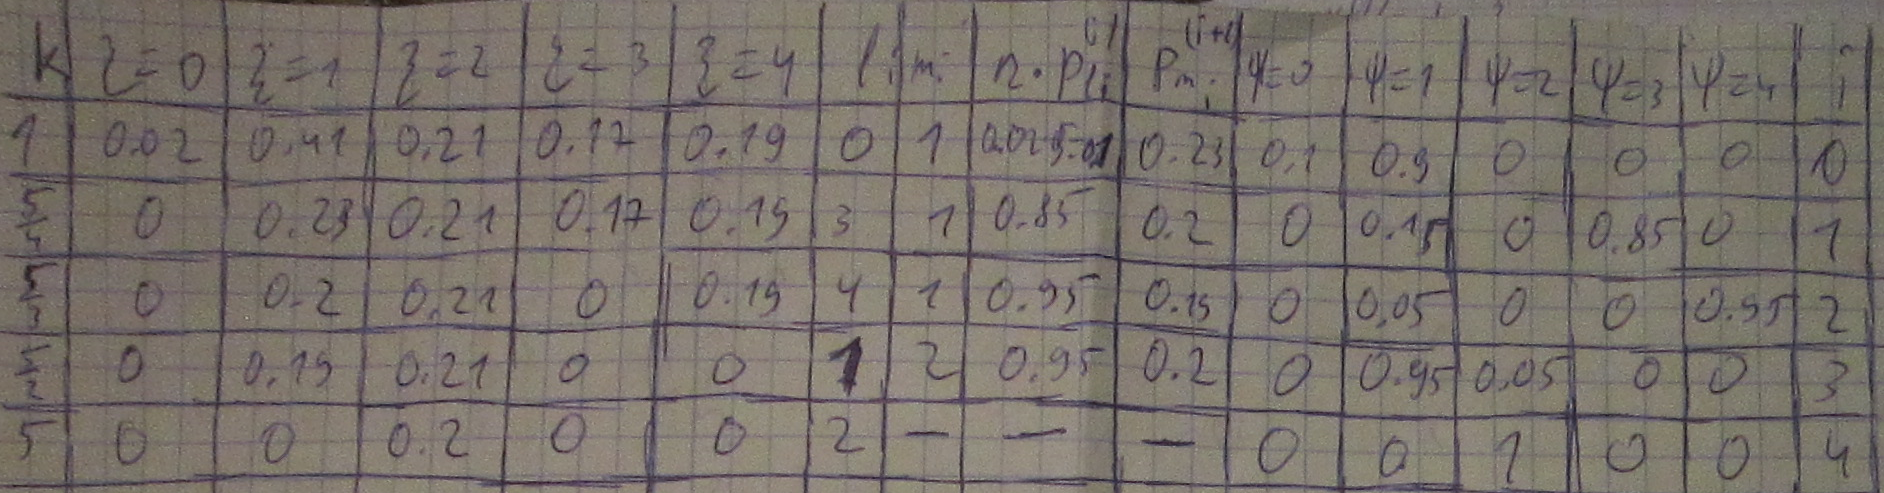
\includegraphics[width=\linewidth]{WalkerTable.png}
\caption{Вычислительная схема}
\label{fig:WalkerTable}
\end{figure}
Следующие 5 столбцов показывают набор вероятностей для $\xi^{(i)}$, затем идут номер $l_i$, номер $m_i$, значение $n * p^{(i)}_{l_i}$, необходимое для построения $\psi^{(i)}$, значение $p^{(i + 1)}_{m_i} = p^{(i)}_{m_i} - \frac{1}{n} + p^{(i)}_{l_i}$ (без домножения на коэффициент!), необходимое для пересчета $\xi^{(i + 1)}$, затем набор вероятностей $\psi^{(i)}$, ну и наконец само i. Здесь стоит заметить, что i - это не только номер текущего шага алгоритма, но и номер базового полуинтервала, который мы на этом шаге алгоритма делим.\\
Как же пользоваться этой схемой? Рассмотрим на примере:\\
Пусть $\alpha_0 = 0.73$. Тогда $n * \alpha_0 = 5 * 0.73 = 3.65$. $\lfloor n * \alpha_0 \rfloor = 3$, значит, мы попали в третий базовый полуинтервал. Граница между полуинтервалами в нем проходит по $n * p^{(i)}_{l_i} = 5 * p^{(3)}_{l_3} = 0.95$. Дробная часть  $\{n * \alpha_0\} = 0.65 < 0.95$, значит, результат эксперимента - $l_i = l_3 = 1$.
\subsubsection{Моделирование ДСВ с помощью последовательности (псевдо)случайных бит.}
Псевдослучайный бит - 0 или 1 равновероятно (бросок монетки).\\
Чего мы хотим? Научиться моделировать ДСВ, вероятности которой - рациональные двоичные числа, с помощью последовательности случайных бит.\\
Пример: $\xi: \; Pr\{\xi = 0\} = \frac{1}{4} = 0.01_2, Pr\{\xi = 1\} = \frac{1}{2} = 0.1_2, Pr\{\xi = 2\} = \frac{1}{4} = 0.01_2$\\
Казалось бы, можно построить полное двоичное дерево нужной глубины h (равной максимальному количеству значащих двоичных цифр после запятой среди $p_i$) и каким-то образом распределить листья по исходам так, чтобы количество листьев, соответствующих i-му исходу было равно $2^h * p_i$. Однако, посмотрим на два различных корректных способа распределения листьев между исходами:\\
\begin{figure}[H]
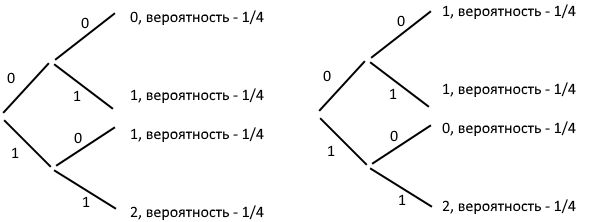
\includegraphics[width=\linewidth]{Bits1.png}
\caption{Сравнение способов}
\label{fig:Bits1}
\end{figure}
В первом случае нам в любом случае придется бросать монетку дважды, а вот во втором если первый бросок монетки выдал результат 0, дальше можно уже не бросать - нам точно известно, что результатом эксперимента будет 1.\\
Собственно, задача изложенного ниже алгоритма в том, чтобы минимизировать среднее число бросков монетки, необходимое для получения результата. Такое разбиение множества листьев будем называть оптимальным.\\
Формализуем:\\
Пусть есть ДСВ $\xi$, $\forall i \in 0:(n - 1) \; Pr\{\xi = i\} = p_i$, $\sum\limits_{i \in 0:(n - 1)}p_i = 1$.\\
$p_i$ в двоичной записи имеет представление $0.\pi^i_1\pi^i_2...\pi^i_m$, то есть $p_i = \frac{\pi^i_1}{2} + \frac{\pi^i_2}{4} + ... + \frac{\pi^i_m}{2^m}$, где $\pi^i_k \in \{0, 1\}$. Тогда $2^mp_i = 2^{m - 1}\pi^i_1 + ... + \pi^i_{m}$.\\
Рассмотрим множество A исходов m бросков монетки. $|A| = 2^m$.\\
Рассмотрим разбиение $A = A_0 \cup A_1 \cup ... \cup A_{n - 1}$, где $\forall i \in 0:(n - 1) \; |A_i| = 2^mp_i$.\\
Тогда если исход эксперимента "m бросков монетки" лежит в $A_i$, то регистрируем исход i. $Pr\{$зарегистрирован исход i$\} = \frac{|A_i|}{2^m} = p_i$. Но как построить оптимальное разбиение?\\
Заведем набор множеств $\forall k \in 1:m \; I_k = \{i \in 0:(n - 1) \; : \; \pi^i_k = 1\}$.\\
Пусть мы бросили монету 1 раз. Множество исходов $B_1$ имеет мощность 2. Выберем какое-то $M_1 \subseteq B_1$ такое, что $|M_1| = |I_1| = \sum\limits_{j \in 0:(n - 1)}\pi^j_1$. Установим биекцию между $M_1$ и $I_1$. Во всех этих случаях исход уже определен, а в остальных $B_1 \setminus M_1$ случаях нам нужно продолжать бросать.\\
Теперь у нас есть $B_2, |B_2| = 2|B_1 \setminus M_1|$, продолжаем использовать тот же алгоритм.\\
В общем случае, у нас есть $B_k$ - множество исходов после k бросков монетки, выбираем из них множество $M_k \subseteq B_k$ исходов такое, что $|M_k| = |I_k|$, строим биекцию между $M_k$ и $I_k$, определяя исход эксперимента для этих случаев, а в остальных $B_k \setminus M_k$ случаях продолжаем бросать.\\
Пример:\\
$p_0 = 0.101001; p_1 = 0.000001; p_2 = 001101; p_3 = 001001$. Тогда:\\
$I_0 = \{0\}$\\
$I_1 = \varnothing$\\
$I_2 = \{0, 2, 3\}$\\
$I_3 = \{2\}$\\
$I_4 = \varnothing$\\
$I_5 = \{0, 1, 2, 3\}$\\
\begin{figure}[H]
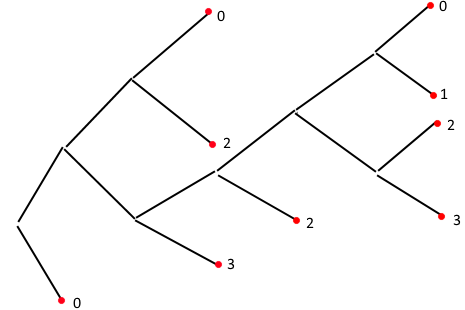
\includegraphics[width=\linewidth]{Bits2.png}
\caption{Дерево вариантов}
\label{fig:Bits2}
\end{figure}
Таким образом, матожидание числа бросков равно:\\
$E\{$число бросков$\} = \sum\limits_{k \in 1:m}k * Pr\{$монета брошена k раз$\} = \sum\limits_{k \in 1:m}k|I_k|\frac{1}{2^k} = \sum\limits_{k \in 1:m}\frac{k}{2^k}\sum\limits_{j \in 0:(n - 1)}\pi^j_k$.
 